% Chapter Template

\chapter{INTRODUCCION} % Main chapter title

\label{C1} % Change X to a consecutive number; for referencing this chapter elsewhere, use \ref{ChapterX}

\lhead{Capítulo 1. \emph{INTRODUCCION}} % Change X to a consecutive number; this is for the header on each page - perhaps a shortened title

%----------------------------------------------------------------------------------------
%	SECTION 1
%----------------------------------------------------------------------------------------

\section{Descripción del problema}
\label{S1_1}

Los estados de agregación clásicos de la materia son tres: sólido, líquido y gaseoso. Los sólidos pueden ser clasificados en metales, cerámicos o polímeros. Esta clasificación se basa en la composición química y la estructura atómica \citep{callister95}. Sin embargo, existe otra clasificación que, en aras de la claridad, suele separarse de los sólidos clásicos: los materiales avanzados. Un material avanzado puede ser un sólido clásico cuyas propiedades han sido mejoradas, pero también puede tratarse de nuevos materiales. En los últimos años, muchos de quiénes trabajan en el área de materiales se han concentrado en la búsqueda de nuevos materiales avanzados \citep{suryana11}. Su clasificación como material avanzado se basa en el uso que se le da: normalmente se trata de aplicaciones que requieren una gran tecnología y para las cuales los sólidos clásicos no siempre son adecuados.

En cuanto a la estructura de los sólidos clásicos, existen aquellos con estructura cristalina y otros con estructura amorfa. La estructura de un sólido se corresponde con el ordenamiento de los átomos en el material. Una estructura cristalina implicaría una disposición de los átomos con ordenamiento tridimensional periódico, formando cristales o granos bien definidos con cierta dirección. Los cristales o granos no son observables a simple vista en metales debido a su naturaleza opaca, pero son evidentes en los minerales \citep{smith96}. Los sólidos amorfos, por el contrario, presentan un ordenamiento de corto alcance o ningún ordenamiento. De los sólidos clásicos, sólo los metales son cristalinos. Tanto los cerámicos como los polímeros presentan estructura amorfa. En la \fref{C1:fg:crystalAmorphous} vemos un ejemplo de sólido amorfo y sólido cristalino.

\begin{figure}[h!]
  \centering
  \begin{tabular}{c}
    \subfloat[Sólido cristalino]{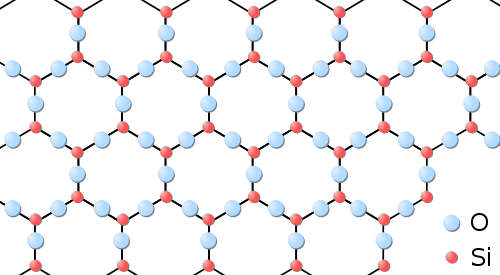
\includegraphics[height=4cm]{Cap_1/500px-SiO2_Quartz.png}}
    \hspace{0.5cm}
    \subfloat[Sólido amorfo]{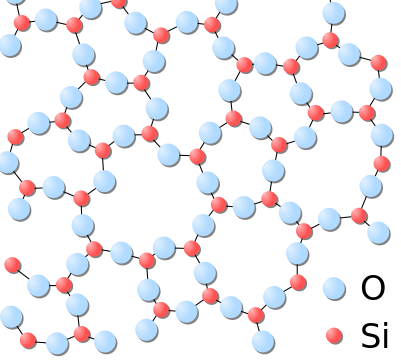
\includegraphics[height=4cm]{Cap_1/500px-Silica.png}}
  \end{tabular}
  \caption[Ejemplo de un sólido cristalinos y un sólido amorfo]{Ejemplo de sólido cristalino (Cuarzo) y sólido amorfo (Vidrio). Ambos casos a partir del Sílice (SiO$_{2}$)}
  \label{C1:fg:crystalAmorphous}
\end{figure}

Por otra parte, en cuanto a la composición química, la clasificación está basada en los elementos químicos que los componen. La tabla periódica de los elementos clasifica a los elementos químicos en elementos metálicos, no metálicos y elementos de transición. Un metal está compuesto de uno o más elementos metálicos (y eventualmente elementos no metálicos en muy baja concentración). Los cerámicos, por otro lado, están compuestos de una mezcla de elementos metálicos y no metálicos. 

\cambio{Estos sólidos, debido a sus diferencias en estructura y composición química, exhiben propiedades mecánicas, térmicas, ópticas, etc. diferentes. Tanto metales como cerámicos suelen contar con una gran rigidez y resistencia. Mientras que los metales se caracterizan por su ductilidad, los cerámicos suelen ser más duros, pero a la vez son más frágiles que los metales y son muy susceptibles a la fractura.} En la \tref{C1:tbl:propiedades} se definen algunas de las propiedades mecánicas que normalmente se estudian en Ciencia de los Materiales.

\begin{table}[htp]
\begin{center}
\begin{tabular}{c C{10cm}}
\hline
\textbf{Propiedades Mecánicas} & \textbf{Definición} \\ \hline
 \hline

Elasticidad &
Capacidad de un material a deformarse ante la acción de una carga, recuperando la forma inicial al retirarse la misma. \\ \hline
 
Plasticidad &
Capacidad de un material a deformarse ante la acción de una carga, permaneciendo la deformación al retirarse la misma. \\ \hline 
 
Resistencia & 
Es la medida de la oposición al cambio de forma, a la destrucción del material. \\ \hline

Dureza & 
Resistencia de la superficie de un material a la penetración por un objeto duro.\\ \hline

Ductilidad & 
Capacidad del material a deformarse de manera permanente (deformación plástica) sin romperse. Un material \textbf{dúctil} es lo opuesto a un material \textbf{frágil}. \\ \hline

Tenacidad & 
Capacidad de un material para resistir cargas de impacto. \\ \hline

Resiliencia &
Capacidad de un material de absorber energía antes de fracturarse. \\ \hline

Maleabilidad & 
Capacidad de un material de deformarse sin romperse obteniendo láminas. \\ \hline

Maquinabilidad &
Propiedad de los materiales que permite comparar la facilidad con que pueden ser mecanizados por arranque de virutas. \\ \hline

Esfuerzo de fluencia & 
Esfuerzo aplicado a un material cuando comienza a evidenciarse una deformación plástica permanente.\\ \hline

Rigidez & 
Medida a través del \textit{Módulo de Young}. Pendiente de la curva tensión-deformación en la región elástica lineal. \\ \hline

Moldeabilidad &
Propiedad de un material de adquirir una forma por efecto de una carga, y de conservarla al retirarse la misma. \\ \hline

\end{tabular}
\end{center}
\caption[Nombre y definición de propiedades mecánicas]{Nombre y definición de propiedades mecánicas normalmente estudiadas en la Ciencia de los Materiales \citep{askeland98}.}
\label{C1:tbl:propiedades}
\end{table}

De lo dicho anteriormente, se observa que tanto los metales como los cerámicos tienen ventajas y deficiencias uno con respecto al otro. Sería lógico entonces intentar combinar ambos tipos de sólido en un único material. Una de las formas de hacerlo es mediante los materiales compuestos. Los materiales compuestos representan una unión macroscópica (e incluso microscópica) heterogénea de uno o más sólidos clásicos como vemos en la \fref{C1:fg:composite}. Sin embargo, cada una de las partes que componen al material compuesto son un sólido clásico. Para lograr una combinación con mejores propiedades es necesario reducir aún más la escala de trabajo, llegando a la escala nanométrica. Un nanómetro es equivalente a $10^{-9} m$. A modo comparativo, el tamaño promedio de un átomo suele tomarse como de 200 pm, lo cual implicaría que un nanómetro contendría 5 átomos.

\begin{figure}[h!]
 \centering
 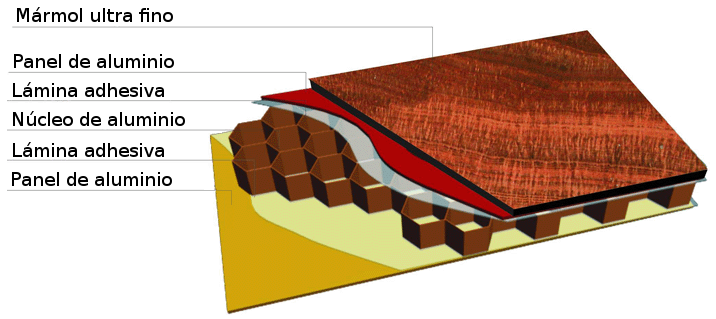
\includegraphics[width=12cm]{Cap_1/composite.png}
 \caption[Esquema de un material compuesto]{Esquema de un material compuesto (adaptado del sitio web de \href{http://www.alustrong.com}{ALUSTRONG}).}
 \label{C1:fg:composite}
\end{figure}

El material denominado vidrio metálico (MG) logra el objetivo de combinar ambos tipos de sólido a escala nanométrica. Se le ha denominado \textit{vidrio} (un material cerámico) debido a su estructura amorfa y \textit{metálico} por tratarse de una aleación de elementos metálicos. Está basado en metales como cobre, níquel, hierro, oro, paladio, titanio, circonio, berilio y lantano; usualmente también se lo combina con bajas proporciones de no metales como boro, silicio, fósforo \citep{andrievski13}.

\cambio{A continuación se sintetizará la teoría detrás de la formación de vidrios metálicos.} Cuando un metal se enfría lentamente, se nuclean pequeños cristales que luego crecen a medida que transcurre el tiempo y que la temperatura baja. Este fenómeno se debe a que el material bajo esas condiciones es más estable bajo una estructura ordenada y periódica, es decir, minimiza su energía libre en un estado de sólido cristalino. Sin embargo, existe otro factor que influencia la solidificación: la dinámica o velocidad de enfriamiento. Al enfriar el líquido a velocidades elevadas, la solidificación es lo suficientemente rápida para mantener la estructura desordenada del líquido, es decir, obtenemos un metal amorfo (o vidrio metálico). El hecho de poder obtener una estructura diferente a la cristalina, implica que existe un equilibrio metaestable para una composición dada a cierta temperatura. Esto sucede cuando la energía libre es un mínimo, pero no un mínimo absoluto.

Teóricamente, todo líquido podría convertirse en vidrio a velocidades de enfriamiento suficientemente altas y temperaturas suficientemente bajas evitando el proceso de cristalización \citep{turnbull61}. A lo largo de los años se han ido perfeccionando varias técnicas que actúan sobre la composición, volumen y velocidad de enfriamiento a la que se somete el material, las cuales han permitido la síntesis de vidrios metálicos.

Una técnica comúnmente usada para lograr que las velocidades de enfriamiento no sean tan extremas es agregar más elementos al vidrio. Es por ello que la mayoría de los MGs que han sido experimentalmente creados son aleaciones de muchos elementos, como por ejemplo el vidrio Pd$_{40}$Cu$_{30}$Ni$_{10}$P$_{20}$. Sin embargo, algunos sistemas binarios también pueden utilizarse. Los MGs basados en metales de transición tardíos (ejemplo Fe, Co, Ni, Cu) presentan ventajas sobre los basados en metales de transición tempranos, como por ejemplo una mayor resistencia y módulo elástico \citep{Xu04}. Por otro lado, los sistemas binarios son útiles para mejorar la eficiencia de formación de MGs, ya que algunos sistemas multicomponentes podrían reducirse a sistemas binarios para su estudio \citep{Duan05}.

Por último, se debe mencionar que un factor limitante en la aplicación industrial de vidrios metálicos es el espesor que es posible obtener para los mismos. Esto se ha visto parcialmente solucionado con la obtención de vidrios metálicos volumétricos, o \textit{Bulk Metallic Glasses} en inglés (BMG). Los BMGs son vidrios metálicos que tienen una sección transversal de por lo menos algunos milímetros de grosor \citep{suryana11}. Es importante que en ninguna parte del material se presenten fases cristalinas, y es por esto que se ha dedicado mucho estudio a la generación de BMGs. Por el hecho de tener un volumen grande, se deben desarrollar nuevas técnicas que permitan una velocidad de enfriamiento lo suficientemente grande como para poder mantener a todo el volumen de material en estado amorfo.

\subsection{Producción de aleaciones metálicas amorfas}
\label{S1_1_1}

Los métodos tradicionales para la preparación de los vidrios metálicos son:

\begin{itemize}
 \item la solidificación del material fundido sobre una superficie en movimiento,
 \item la deposición en substratos fríos,
 \item y la electrodeposición.
\end{itemize}

Pol Duwez propuso un método para obtener una lámina de metal amorfo a partir de un líquido que pasa a través de dos grandes ruedas de cobre a baja temperatura \citep{duwez60}. Al ser pequeña la relación entre la superficie de contacto del líquido y el volumen, éste se enfría de manera casi instantánea. En un proceso similar denominado Torneado en estado de fusión (o \textit{Melt Spinning} en inglés, ver \fref{C1:fg:meltSpinning}) se utiliza un sólo disco giratorio sobre el que se hace impactar un chorro líquido a alta presión sobre la cara exterior de la rueda, logrando velocidades de enfriamiento de hasta $10^{7}$ K/s.

\begin{figure}[h!]
  \centering
  \begin{tabular}{c}
    \subfloat[Maquinaria]{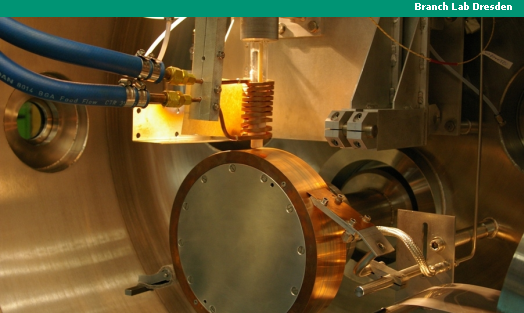
\includegraphics[height=4cm]{Cap_1/melt_spinning_A.png}}
    \vspace{1cm}
    \subfloat[Proceso]{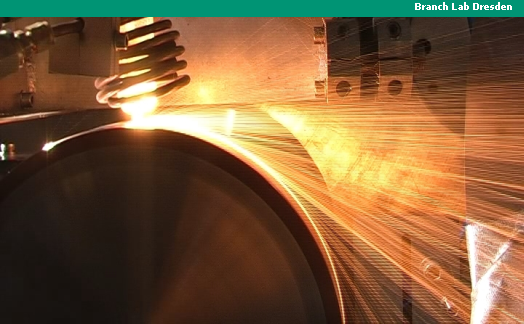
\includegraphics[height=4cm]{Cap_1/melt_spinning_B.png}}
  \end{tabular}
  \caption[Torneado en estado de fusión]{Imágenes del proceso de \textit{Melt Spinnning} (del sitio web del \href{http://www.ifam.fraunhofer.de/en/Dresden/Sintered_and_Composite_Materials/Nanostrukturierte_Werkstoffe.html}{IFAM}, Fraunhofer Institute for Manufacturing Technology and Advanced Materials).}
  \label{C1:fg:meltSpinning}
\end{figure}

Otra opción es atomizar un líquido y enfriar las pequeñas gotas mediante un gas. Se puede obtener así polvo de vidrio metálico (el cual es necesario sinterizar sin perder las propiedades inducidas por el enfriamiento), o hacer impactar estas gotas contra un molde para crear un sólido de forma directa. Existen métodos comerciales que logran una porosidad tan baja que el material así formado puede luego ser forjado. En la \fref{C1:fg:metal_powder} podemos ver un esquema del proceso de atomizado. En particular, se puede observar el proceso conocido como \textbf{\textit{VIGA}} (la sigla significa \textit{\textbf{V}acuum \textbf{I}nduction melting combined with \textbf{G}as \textbf{A}tomization} o fundido por inducción al vacío combinado con atomización por gas) y el \textbf{\textit{EIGA}} (la sigla significa \textit{\textbf{E}lectrode \textbf{I}nduction melting combined with \textbf{G}as \textbf{A}tomization} o fundido por inducción de electrodo).

\begin{figure}[h!]
 \centering
 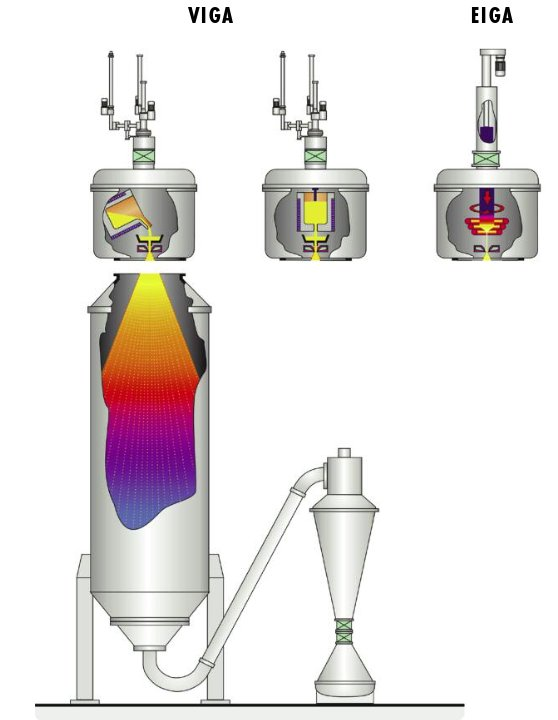
\includegraphics[width=10cm]{Cap_1/metal_powder.jpeg}
 \caption[Atomizado de metal]{Esquema del atomizado de partículas líquidas de una aleación (de ALD Vacuum Technologies \href{www.ald-vt.de}{www.ald-vt.de})}
 \label{C1:fg:metal_powder}
\end{figure}

Si bien el principio es el mismo, la calidad de la aleación resultante de estos procesos depende fuertemente de la composición del material utilizado, ya que esta afecta en gran medida la capacidad de formación de vidrio del material. Teniendo en cuenta que la extracción rápida de calor de un material es una operación difícil, es de interés encontrar composiciones que permitan producir vidrios a menores velocidades de enfriamiento.

\subsection{Propiedades y aplicaciones de los vidrios metálicos}
\label{S1_1_2}

Como ya se ha dicho, los vidrios metálicos poseen características y propiedades excepcionales que los hacen candidatos para ser usados en artefactos tecnológicos modernos o de alta complejidad.

La \tref{C1:tbl:props} es una adaptación de un estudio realizado por \cite{ashby06}, en el cual se analizan las propiedades de los vidrios metálicos para su posible aplicación como materiales estructurales.

\begin{table}[htp]
\begin{center}
\begin{tabular}{c C{5cm} C{5cm}}
\hline
\textbf{Atributos} & \textbf{Ventajas} & \textbf{Desventajas} \\ \hline
 \hline

Generales &
Ausencia de efectos adversos debidos a fronteras de granos. &
Alto costo y grandes limitaciones de fabricación \\ \hline
 
Mecánicos &
Alta dureza. Resistencia al desgaste y la abrasión. Gran resistencia mecánica y menor rigidez que las aleaciones cristalinas. Esto le provee una muy alta resiliencia. & 
Gran pérdida de ductilidad ante la aparición de bandas de corte (véase \sref{S1_1_3}). El recocido (\textit{annealing} en inglés) lo vuelve frágil. \\ \hline 
 
Térmicos & 
Su baja temperatura de transición vítrea ($T_g$) permite el tratamiento como líquido superenfriado. & 
Presenta inestabilidad a temperaturas altas (superiores a $T_g$). \\ \hline

Eléctricos y magnéticos & 
Alta permeabilidad magnética. La resistividad es casi independiente de la temperatura.& 
En campos oscilantes se pierde energía, al ser un material magnetoestrictivo (como aquellos utilizados en transductores).\\ \hline

Químicos & 
Resistencia a la corrosión debido a la falta de bordes de grano.& \\ \hline

Ambientales & 
Algunos MG son biocompatibles & No son fáciles de reciclar. \\ \hline

\end{tabular}
\end{center}
\caption[Propiedades de los vidrios metálicos]{Propiedades de los vidrios metálicos (adaptada de la tabla en \cite{ashby06}).}
\label{C1:tbl:props}
\end{table}

\begin{figure}
 \centering
 \begin{tabular}{cc}
 \subfloat[Hoja quirúrgica de material estándar]{
    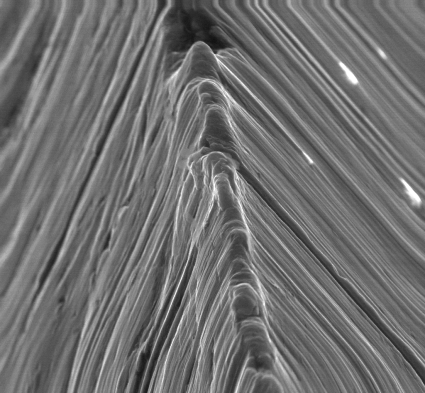
\includegraphics[height=4cm]{Cap_1/blade.png}
    \label{C1:fg:blade}}
  &
  \subfloat[Hoja quirúrgica de BMG]{
    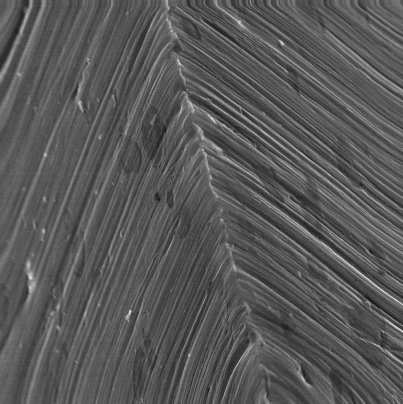
\includegraphics[height=4cm]{Cap_1/BMG-blade.png}
    \label{C1:fg:bladeBMG}} \\
  \subfloat[Omega Seamaster Edición Limitada]{
    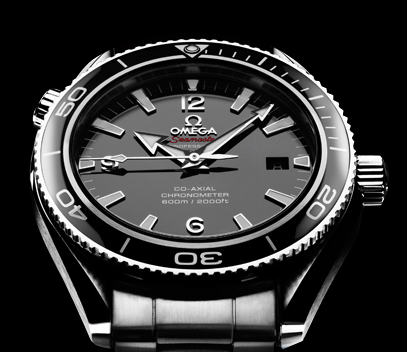
\includegraphics[height=4cm]{Cap_1/seamaster.png}
    \label{C1:fg:seamaster}}
  &
  \subfloat[Recubrimientos en palos de Golf]{
    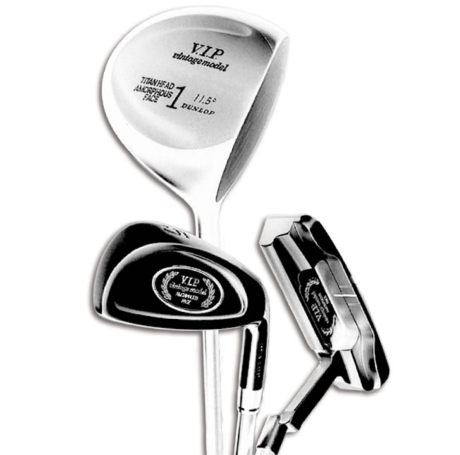
\includegraphics[height=4cm]{Cap_1/golf.png}
    \label{C1:fg:golf}}\\
  \subfloat[MEMS]{
    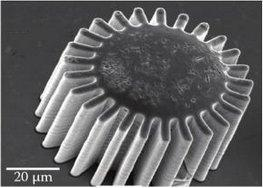
\includegraphics[height=4cm]{Cap_1/MEMS_A.jpeg}
    \label{C1:fg:mems_A}}
  &
  \subfloat[MEMS]{
    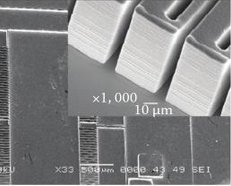
\includegraphics[height=4cm]{Cap_1/MEMS_B.jpeg}
    \label{C1:fg:mems_B}}  
 \end{tabular}
  \caption[Aplicaciones de BMGs]{Algunos ejemplos de usos actuales de vidrios metálicos. Las Figuras~\ref{C1:fg:blade} y \ref{C1:fg:bladeBMG} son imágenes obtenidas a partir de SEM que comparan el filo de un elemento quirúrgico estándar contra uno basado en BMGs.}
  \label{C1:fg:usecases}
\end{figure}

Es evidente del análisis de la tabla que los vidrios metálicos, en el estado actual de la técnica, sólo son viables en aplicaciones de alto valor agregado, dado su alto costo de fabricación. Por otro lado, hasta que no se mejoraron las técnicas de fabricación no fue posible obtener vidrios metálicos de volúmenes considerables. Por ello las aplicaciones comerciales ``tradicionales'' de estos materiales fueron como revestimiento (debido a su resistencia a la corrosión, el desgaste y las ralladuras), y en transformadores, dando blindaje magnético (debido a las excelentes propiedades magnéticas de los vidrios metálicos basados en hierro).

Con el surgimiento de nuevas técnicas de fabricación, el interés en estos materiales ha resurgido y las aplicaciones han aumentado en cantidad. Son ampliamente usados en equipamiento deportivo de primera calidad, debido a su relación resistencia-peso y a su gran resiliencia. Estas características permiten que se gaste muy poca energía en la deformación del material y que más energía se transmita.

La biocompatibilidad de algunos vidrios metálicos los hace candidatos para ser utilizados en aplicaciones biomédicas. Otros usos posibles son: sistemas microelectromecánicos (MEMS), electrónica de consumo, aplicaciones aeroespaciales, etc. En la \fref{C1:fg:usecases} se muestran algunos de las aplicaciones que se han detallado en la presente sección.

\subsection{Mecánica de la deformación de vidrios metálicos}
\label{S1_1_3}

Una de las mayores limitaciones para el uso de los vidrios metálicos en aplicaciones estructurales está relacionado con su mecánica de deformación. Debido a su estructura amorfa, los vidrios metálicos, a diferencia de las aleaciones cristalinas, no se endurecen con la deformación, sino que les ocurre exactamente lo contrario en un proceso denominado ablandamiento por deformación (\textit{strain softening} en inglés). Este debilitamiento resulta en la concentración de deformación en bandas muy estrechas, llamadas \textbf{bandas de corte} (SB, por sus siglas en inglés). El crecimiento de estas bandas puede causar la fractura frágil del material \citep{schuh07}. En la \fref{C1:fg:shearbands} se puede observar una muestra en la que aparecen SBs luego de haber sido traccionada a una velocidad de deformación $d\epsilon/dt=4\cdot10^7s^{-1}$ a distintas temperaturas.

\begin{figure}[H]
 \centering
 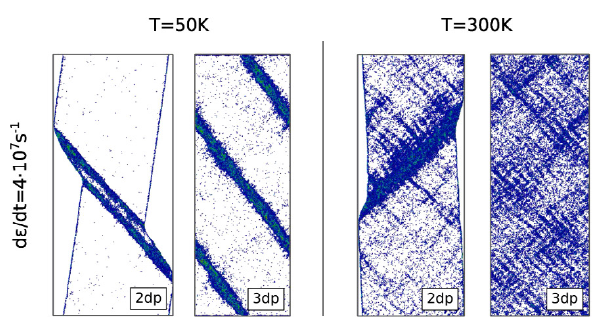
\includegraphics[width=10cm]{Cap_1/shearbands.png}
 \caption[Bandas de corte]{Muestra de BMG bajo tracción uniaxial a $\epsilon$=18\%. Adaptado de \cite{albe13}}
 \label{C1:fg:shearbands}
\end{figure}

Varias teorías se han desarrollado en el intento de explicar este fenómeno. Tal vez la más aceptada actualmente es la teoría de zonas de transformación de tensión cortante (STZ por sus siglas en inglés: \textit{shear transformation zones}). Las STZ son pequeñas regiones de pocos átomos cuyo posicionamiento y configuración los hace susceptibles a deformaciones plásticas en respuesta a esfuerzos de corte.

Los conceptos fundamentales de la teoría de STZs fueron desarrollados por Argon \citep{argon79}. Luego Falk y Langer \citep{Falk98, Langer07} desarrollaron una teoría dinámica de STZs (ver \fref{C1:fg:stzs}). En este modelo, ciertas zonas de pocos átomos pueden deformarse plásticamente y quedarse bloqueadas en este estado deformado, sin poder seguir deformándose en la misma dirección. La formación de STZs puede llegar a ocurrir a iguales velocidades que el bloqueo de las mismas, y bajo esta condición ocurre flujo plástico.

La acumulación de STZs en ciertas direcciones de corte principales produce las bandas de corte (SB).

\begin{figure}[H]
 \centering
 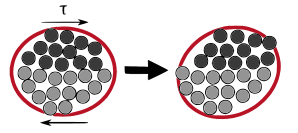
\includegraphics[width=7cm]{Cap_1/stzs.png}
 \caption[Zonas de transformación de tensión cortante]{Zonas de transformación de tensión cortante (STZ). Adaptado de \cite{albe13}}
 \label{C1:fg:stzs}
\end{figure}

%----------------------------------------------------------------------------------------
%	SECTION 2
%----------------------------------------------------------------------------------------

\section{Antecedentes}
\label{S1_2}

Podemos decir que a grandes rasgos en la producción científica en torno a los vidrios metálicos se distinguen tres enfoques de trabajo:

\begin{itemize}
 \item el modelado de las diferentes propiedades a nivel físico-matemático,
 \item la descripción de comportamientos bajo diferentes condiciones de ensayo,
 \item y la mejora de las propiedades mecánicas.
\end{itemize}

A continuación se resume la producción científica de los últimos años que sirven de base para este trabajo. Hay que tener presente que algunos de los estudios se realizan mediante simulación, otros experimentalmente y otros con ambos métodos a modo de validación.

\subsection{Modelado de vidrios metálicos}
\label{S1_2_1}

Ciertos estudios intentan describir matemáticamente las deformaciones y los esfuerzos máximos de los MGs, en situaciones ideales de régimen plástico homogéneo \citep{Wisitsorasak12, cheng11}. La mecánica de falla de estos materiales es también estudiada ya que en el caso general la plasticidad se presenta de manera abrupta causando la falla inesperada \citep{Chen11, Egami11}.

La mecánica de cavitación es estudiada por diversos autores describiendo la nucleación y crecimiento de los poros como desencadenantes de las fallas en MGs \citep{Huang13, guan13}. Gao \citep{Gao14} modela y analiza las interfaces amorfo-cristalinas en profundidad con un enfoque en describir los poliedros de Voronoi como indicadores del ordenamiento atómico local.

\subsection{Descripción de comportamiento}
\label{S1_2_2}

Xiao \citep{xiao12} observa la mecánica de deformación de MGs en nano-alambres bajo compresión, y cómo la velocidad de enfriamiento afecta la formación de bandas de corte. Un estudio de la tolerancia al daño de los MGs lleva a indicar que la relación dureza-resistencia de los mismos es comparable a la de los materiales más resistentes conocidos \citep{Demetriou11}.

Nos encontramos también con ensayos de nano-alambres, en donde la dependencia de la resistencia y la ductilidad con el tamaño de muestra se analizan realizando ensayos de tracción en aleaciones basadas en circonio de diferente diámetro junto con ciclos de carga y descarga \citep{Dongchan10}.

En un esfuerzo por comprender la dinámica de los átomos de mayor energía de deformación (\textit{atomic strain energy}) se compara la evolución de los desplazamientos cuadráticos medios entre estos y el de todos \citep{tang15}. El hecho de que su dinámica sea distinta se ve correlacionada con la respuesta esfuerzo-deformación de los mismos, lo que podría sugerir una relación con la nucleación de STZs y la posterior propagación en SBs. Esta relación también es estudiada desde otro enfoque en ensayos de nano-indentación \citep{gu15}, donde se estudia la deformación plástica durante el ensayo, observando la propagación de bandas de corte embrionarias (ESBs) sin la formación de bandas de corte maduras (MSBs) que propaguen a través del material en su totalidad. El fenómeno es atribuido a los tamaños de muestra utilizados, ya que según Shimizu \citep{shimizu06} existe una escala de longitud intrínseca de unos 100 nm por debajo de la cual la concentración de esfuerzo de corte en la escala de la muestra no ocurre a menos que se utilicen velocidades de deformación muy elevadas (> 10$^{8}$/s), como encontramos comúnmente en simulaciones de MD.

Al someter a esfuerzos (ya sean uniaxiales, compuestos, y/o repetitivos) podemos encontrarnos con ciertas zonas del material que almacenan la energía necesaria para un cambio de fase, y pasar a una fase cristalina. Mao \citep{ma15} estudia la transición amorfo-cristal al someter una muestra de aluminio-hierro (Al$_{50}$Fe$_{50}$) a esfuerzos fluctuantes de tracción. Lo que se observa es que si bien el ensayo se realiza a temperaturas bajas (50 K) partes del material cristalizan luego de cierto número de ciclos. Es interesante este efecto ya que podría darse por sentado que solo a altas temperaturas podríamos encontrarnos con estos efectos (cuando la cristalización ocurre a causa de la difusión activada térmicamente) y por consiguiente encontrarnos ante situaciones de falla inesperada.

\subsection{Mejora de propiedades mecánicas}
\label{S1_2_3}

Para controlar y por consiguiente mejorar la dinámica de la plasticidad, se ha modificado tanto la composición como la estructura a escala nano y micro de los vidrios metálicos de diferentes maneras. Cada investigación presenta un enfoque diferente de los mecanismos de deformación según el objetivo del estudio. A veces la generación de SBs se considera deseable (siempre y cuando sean controladas): \cite{chen14} se benefician de las deformaciones plásticas y las micro-fracturas para la disipación de energía y así pensar en su aplicación a dispositivos de absorción de energía.

Por otro lado, muchos trabajos se centran en impedir la propagación de SBs para evitar que el material falle de manera frágil y no controlada. Particularmente, la inclusión de nanopartículas cristalinas provee obstáculos a la propagación y crecimiento de SBs. Esto se traduce en una deformación más reducida y homogénea en régimen plástico. Albe \citep{albe13} estudia a través de MD los efectos de agregar numerosos nanoprecipitados de cobre cristalino en una matriz amorfa. En este caso las simulaciones se realizan a bajas temperaturas (50 K) y relativamente bajas velocidades de deformación (10$^{7}$ /s).

Los mecanismos de propagación de SBs en un medio con nanopartículas embebidas son estudiados en otro trabajo con más detalle \citep{brink15}. En el mismo se señala que el tamaño de la inclusión, el esfuerzo necesario para crear dislocaciones en la misma, y la distancia entre precipitados juegan roles conjuntos cuando una SB se propaga. Notan cuatro mecanismos: la partícula se disuelve a estado amorfo por el esfuerzo cortante, la SB rodea a la partícula y sigue su camino, la nanopartícula bloquea el paso de la SB y se nuclea en una dirección diferente, la SB corta la nanopartícula produciendo dislocaciones internas. En este trabajo también se analizan casos experimentales a través de Microscopia Electrónica de Transmisión (TEM).

Por otra parte, el agregado de precipitados modifica la plasticidad inducida por deformación \citep{kuo14}. Un método para introducir estos precipitados en la matriz amorfa es la formación mediante recocido. En el trabajo de \cite{wei14} primero se obtiene una matriz amorfa de MG y luego se la recoce alrededor de la temperatura de transición $T_{g}$ para lograr cristalizar estructuras $B2$ en una proporción cercana a la deseada.

Otra de las formas de obstaculizar la propagación de SBs que ha suscitado interés últimamente es la nanoporosidad. \cite{wang10} estudian mediante MD los efectos de nanoporos sobre la resistencia y ductilidad de un vidrio metálico durante ensayos de compresión uniaxial y nanoindentación. Notan que, si bien los poros sirven como concentradores de tensión y actúan como catalizadores de SBs, su posterior colapso incrementa la resistencia del material, dificultando la propagación de dichas bandas de corte. A su vez, la presencia de poros produce una reducción de la resistencia a la fluencia y del límite elástico. También notan que el tamaño de los poros tiene gran influencia en la resistencia última al corte, siendo ésta mayor cuando hay poros de mayor tamaño. \cite{yuan14} estudian la dependencia que guardan ciertas propiedades mecánicas con el tamaño de los poros y la densidad relativa del material. \cite{sarac14} estudian la misma dependencia mediante un modelo mecánico a escala del continuo.

Los efectos del cambio en la composición son estudiados por \cite{Zheng12}, donde el incremento de ductilidad se asocia al reemplazo de átomos por otros diferentes, modificando las propiedades de los enlaces atómicos.

%----------------------------------------------------------------------------------------
%	SECTION ???
%----------------------------------------------------------------------------------------

%\section{Muestra de vidrio metálico: Cobre-Circonio. ESTA SECCION HAY Q CAMBIARLA. LA DEJO PARA COPIAR}
%\label{S123456}

%La muestra que se utilizará y servirá de base para otras muestras es una muestra de un vidrio binario, más específicamente \CuZr (Cobre-Circonio), que se manipulará para simular un BMG (Bulk Metallic Glass por sus siglas en inglés). Aquí es necesario explicar los conceptos de BMGs y vidrios binarios de base Cobre.


%----------------------------------------------------------------------------------------
%	SECTION 3
%----------------------------------------------------------------------------------------

\section{Alcances de este trabajo}
\label{S1_3}

En este trabajo nos avocaremos al estudio del régimen elasto-plástico con grandes deformaciones de vidrios metálicos sometidos a esfuerzos de tracción y compresión, el análisis de parámetros constitutivos y modificaciones estructurales que impacten en su comportamiento mecánico, como así también la influencia de la temperatura.

Nos centraremos en una muestra de cobre-circonio (\CuZr) para la cual se emplea un potencial interatómico descrito correctamente \citep{daw84} y utilizado ampliamente en la literatura \citep{shimizu07,cao09,cheng09,arman10,cheng11,wang12}. Los ensayos realizados presentan un sentido y velocidad de deformación constante, es decir, no se realizan ensayos de carga cíclicos. En el caso general, se aplican condiciones de borde periódicas a la muestra en tres dimensiones y adicionalmente se realizan ensayos con condiciones de borde libres para comparaciones específicas.

Además se analiza la respuesta mecánica de vidrios metálicos con inclusiones de nanopartículas como así también con nanoporos.

Por último, los estudios aquí presentados son realizados mediante experimentos numéricos a escala nanométrica.


%----------------------------------------------------------------------------------------
%	SECTION 4
%----------------------------------------------------------------------------------------

\section{Objetivos}
\label{S1_4}

A continuación se detallan los objetivos de este trabajo de investigación:

\begin{itemize}
 \item Investigar el comportamiento en régimen elasto-plástico en grandes deformaciones de un metal amorfo binario a diferentes temperaturas.
 \begin{itemize}
  \item Analizar los esfuerzos y deformaciones en régimen elasto-plástico.
  \item Estudiar el comportamiento frente a la temperatura de diferentes parámetros.
  \item Estudiar el comportamiento de las bandas de corte y buscar posibles soluciones para evitar o retardar la falla frágil.
 \end{itemize}
 \item Investigar los efectos de cambios en la composición de la muestra sobre las propiedades mecánicas.
 \begin{itemize}
  \item Generar nuevas muestras modificadas: muestras de porosidad variable y muestras con inclusiones cristalinas.
  \item Analizar el comportamiento general de la muestra modificada bajo esfuerzos, a diferentes temperaturas.
  \item Analizar el comportamiento particular de las inclusiones/poros sometidos a esfuerzos, a diferentes temperaturas.
 \end{itemize}
 \item Resumir el know-how adquirido en un documento que permita una incorporación más rápida a los proyectos de investigación que estén relacionados a la temática abordada.
\end{itemize}

%----------------------------------------------------------------------------------------
%	SECTION 5
%----------------------------------------------------------------------------------------

\section{Metodología}
\label{S1_5}

Para alcanzar los objetivos propuestos en este trabajo se hace uso de Dinámica Molecular. Para ello, en primer lugar es necesario:

\begin{itemize}
 \item Comprender la metodología de las simulaciones de Dinámica Molecular,
 \begin{itemize}
  \item estudiar los principios de dichas simulaciones,
  \item y comprender las técnicas de pre/post procesamiento de la información obtenida.
 \end{itemize}
\end{itemize}

En particular, se hace uso de simulaciones de MD mediante el paquete LAMMPS \citep{plimpton95}, que es de código abierto y gratuito. Se prepara un script de entrada que describe la simulación (ver \aref{AA}) y una vez comprobado que su ejecución es correcta, se generan copias con parámetros diferentes, como por ejemplo la temperatura de simulación.

A partir de la ejecución de las simulaciones, se generan dos tipos de archivos de salida. Por un lado tenemos una salida de variables termodinámicas, es decir, cómputos promedios de la muestra completa como la temperatura, la energía potencial, las dimensiones y las componentes del tensor de esfuerzos. Se los denomina generalmente archivos \textit{out} o \textit{log}. Por otro lado nos encontramos con archivos que contienen propiedades similares pero para cáda átomo. Estos últimos son de un tamaño considerablemente mayor y representan el comportamiento atómico en detalle, ya que contienen información de las posiciones, velocidades, tensor de esfuerzo y energías. Se los denomina arhivos \textit{dump}.

Sobre los archivos \textit{out} es necesario realizar un post-procesamiento para calcular variables determinadas (por ejemplo la tensión de Von Mises) antes de pasar a una representación gráfica. Los archivos \textit{dump} son tratados de manera similar, pero se representan mediante un  software dedicado, que en nuestro caso es Ovito \citep{stukowski10} (ver \aref{AB}).

%----------------------------------------------------------------------------------------
%	SECTION 6
%----------------------------------------------------------------------------------------

\section{Contenidos}
\label{S1_6}

El presente trabajo se divide en cinco capítulos y cuatro apéndices. Una presentación teórica se encuentra en el \cref{C2}. Los Capítulos \ref{C3} a \ref{C5} engloban los resultados obtenidos, presentando cada uno de los diferentes casos de análisis. Las conclusiones finales pueden encontrarse en el \cref{C6}. Los Apéndices \ref{AA} a \ref{AD} dan una introducción a las herramientas utilizadas en este trabajo.

En particular el \cref{C2} presenta los fundamentos teóricos de las simulaciones de MD, gracias a las cuales se pueden realizar nuestros ensayos computacionales. Se muestran algunos algoritmos utilizados internamente por LAMMPS y las ecuaciones que describen las interacciones atómicas de nuestra muestra.

El \cref{C3} detalla los resultados obtenidos al simular una muestra de \CuZr bajo diferentes modos de carga y temperaturas. Se obtienen curvas de esfuerzo-deformación, módulo de Young y tensión máxima contra temperatura, entre otros.

En el \cref{C4} se analiza la estabilidad de nanopartículas cristalinas embebidas en la matriz amorfa original. Se realizan cálculos de difusividad del cristal en la matriz y se compara el comportamiento mecánico de la muestra con este agregado frente a las respuestas sin nanopartículas cristalinas embebidas.

En el \cref{C5} se estudia la mecánica de deformación y de cierre de los poros en una matriz de porosidad variable, así como la respuesta mecánica de la muestra en su totalidad frente a la matriz amorfa sin nanoporos. 

El \aref{AA} contiene los lineamientos generales para la compilación y utilización del software de simulación elegido (LAMMPS). En el \aref{AB} se describe el modo de uso del software de visualización Ovito. En el \aref{AC} se da una pequeña introducción a técnicas de \textit{scripting} para pre y post procesamiento de datos de salida. Finalmente, en el \aref{AD} se presentan algunos de estos scripts y otros scripts de automatización de tareas.